%!TeX root=../tese.tex
%("dica" para o editor de texto: este arquivo é parte de um documento maior)
% para saber mais: https://tex.stackexchange.com/q/78101/183146

%% ------------------------------------------------------------------------- %%
\chapter{Implementação do Projeto}
\label{cap:Implementação}

Agora que foram definidas as mecânicas de jogo do ponto de vista de um jogador e
explicado que uma das intenções do projeto é facilitar o aprendizado de um 
iniciante em computação é preciso explicar melhor os detalhes da implementação
para concluir a segunda intenção do projeto que é permitir a extensão do jogo
por alguém que já conheça um pouco de programação ou esteja interessado em 
modificar o código fonte, inserindo novas funcionalidades. 

Para isso, essa seção divide a explicação dos arquivos do jogo agrupando por 
funcionalidades, assim entender o código de implementação torna-se mais simples.

\section{Inventário}

Dentro dos arquivos do jogo (diretório \textit{Phoenix Rising}) é encontrado na 
pasta \textit{GenericGameScenes} e administra os comandos disponíveis e a
movimentação deles na tela.

A seguir estão imagens com os nós que compõem a cena, os métodos do script
atrelado ao nó raiz, chamado \textit{Inventory} e as variáveis mais importantes
para entender o código.

\begin{minipage}[c]{0.5\textwidth}
    \begin{figure}[H]
        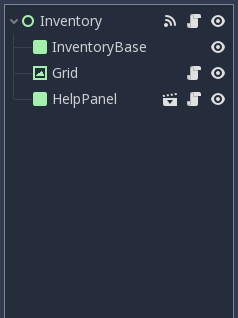
\includegraphics[scale=0.6]{../figuras/cena_inventory.png}
        \caption{Árvore da cena Inventory}
    \end{figure}
\end{minipage}%
\begin{minipage}[c]{0.5\textwidth}
    \begin{figure}[H]
        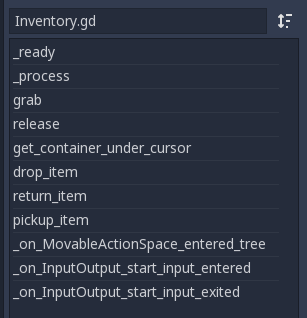
\includegraphics[scale=0.6]{../figuras/funcoes_inventory.png}
        \caption{Funções do script do nó Inventory}
    \end{figure}
\end{minipage}

\begin{figure}[H]
    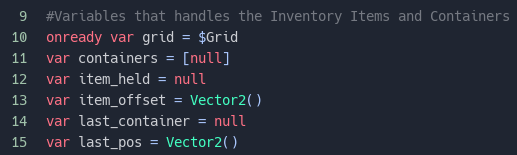
\includegraphics[scale=0.7]{../figuras/variaveis_inventory.png}
    \caption{Variáveis do script do nó Inventory}
\end{figure}

O nó \textit{InventoryBase} apenas dá cor ao espaço destinado aos comandos no
início do jogo e o nó \textit{HelpPanel} é uma cena instanciada que gerencia o
menu de ajuda que aparece ao solicitar mais explicações sobre um comando.

Dentro do jogo \textit{Phoenix Rising} os comandos disponíveis devem ocupar o
espaço de áreas específicas. Estas áreas são chamadas de recipientes (do 
inglês \textit{container}). Um recipiente pode ser o próprio \textit{Grid} do 
inventário ou espaços definidos dentro dos Espaços de Ação, que serão explicados
posteriormente.

O nó \textit{Grid} tem grande importância dentro da cena, pois é ele quem separa
cada recipiente da tela de jogo em pequenos quadradinhos, facilitando a mecânica
de mover os comandos disponíveis. Estes recipientes são adicionados na lista de 
\textit{containers}, definida na linha 11 da figura 3.3.

Para facilitar o entendimento, veja as variáveis mais importantes e o método de 
inicialização da grade (do inglês \textit{grid}):

\begin{minipage}[c]{0.5\textwidth}
    \begin{figure}[H]
        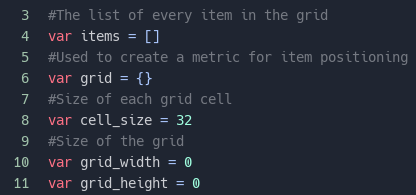
\includegraphics[scale=0.5]{../figuras/grid_variables.png}
        \caption{Variáveis do Grid}
    \end{figure}
\end{minipage}%
\begin{minipage}[c]{0.6\textwidth}
    \begin{figure}[H]
        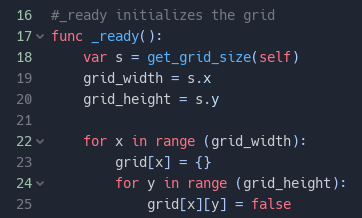
\includegraphics[scale=0.6]{../figuras/grid_ini.png}
        \caption{inicialização do Grid}
    \end{figure}
\end{minipage}

O tamanho de cada quadrado é armazenado e definido na linha 8 da figura 3.4
e as medidas da grade são armazenadas pelas variáveis definidas nas linhas
10 e 11 da mesma figura.

Na inicialização da grade do inventário o método \textit{get\_grid\_size} 
recebe o retângulo que foi definido para ser o recipiente e devolve seu 
tamanho (largura e altura) usando o sistema quadriculado, ou seja, devolve 
quantos quadrados de largura e altura ele ocupa. Depois, cada posição 
desta grade recebe o valor "falso", sinalizando que aquele quadrado está vazio,
ou seja, que nenhum item do jogo ocupa aquelas posições.

A partir dessa divisão todo comando que é disponibilizado no inventário ocupará
um número de quadrados do \textit{grid} e a movimentação destes itens é feita 
pelos métodos de pegar (do inglês \textit{grab}) e soltar (do inglês 
\textit{release}) definidos no \textit{scripts} do nó \textit{Inventory}. Ao
posicionar um comando em alguma região do recipiente os quadrados são marcados
com "verdadeiro" para sinalizar que aquela região está preenchida.

\begin{figure}[H]
    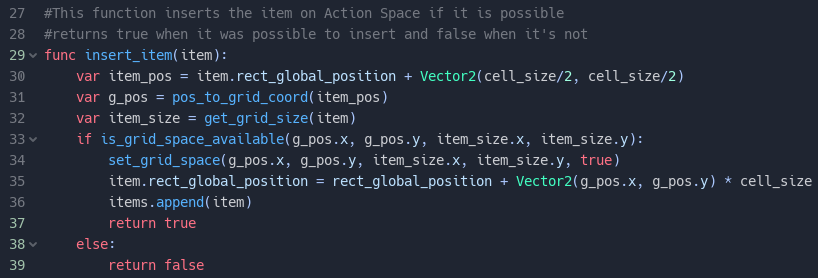
\includegraphics[scale=0.6]{../figuras/insere_item.png}
    \caption{Método de inserção de um item}
\end{figure}

\begin{figure}[H]
    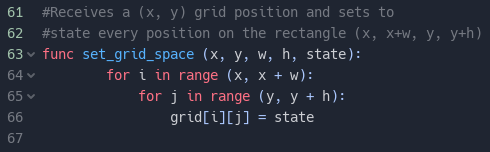
\includegraphics[scale=0.7]{../figuras/marca_grid.png}
    \caption{Marcação das posições do grid}
\end{figure}

\section{Espaço de Ação}

Dentro dos arquivos do jogo (diretório \textit{Phoenix Rising}) é encontrado na 
pasta \textit{ActionSpace}. O espaço de ação serve para conectar o sistema
fazendo com que seja possível executá-lo e posicionar os comandos que serão
utilizados no programa criado pelo jogador.

Basicamente o espaço de ação é divido em duas partes, uma móvel e outra fixa.
A cena \textit{MovableActionSpace} é a parte que permite a mobilidade e a cena
\textit{ActionSpace} cuida de receber o item posicionado e os argumentos.

\begin{minipage}[c]{0.5\textwidth}
    \begin{figure}[H]
        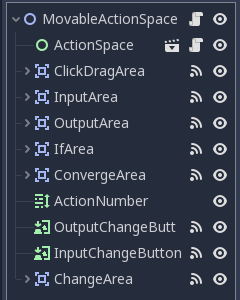
\includegraphics[scale=0.8]{../figuras/cena_movable_action_space.png}
        \caption{Cena MovableActionSpace}
    \end{figure}
\end{minipage}%
\begin{minipage}[c]{0.6\textwidth}
    \begin{figure}[H]
        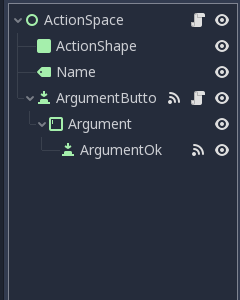
\includegraphics[scale=0.8]{../figuras/cena_action_space.png}
        \caption{Cena ActionSpace}
    \end{figure}
\end{minipage}

Note que, como \textit{MovableActionSpace} é móvel, foi utilizado um nó do tipo
Node2D e como \textit{ActionSpace} é fixo, foi utilizado um nó do tipo Control.

A cena \textit{MovableActionSpace} é formada pelos seguintes nós:

\begin{itemize}
    \item[$\bullet$]
        \textbf{\textit{ActionSpace}} - Cena que trata dos comandos e argumentos
        que são posicionados para a execução.   
    \item[$\bullet$]
        \textbf{\textit{ClickDragArea}} - Área com o ícone da mãozinha, 
        destinada a mover o espaço de ação pela tela. 
    \item[$\bullet$]
        \textbf{\textit{InputArea}} - Conexões simples de \textit{input}.
    \item[$\bullet$]
        \textbf{\textit{OutputArea}} - Conexões simples de \textit{output}.  
    \item[$\bullet$]
        \textbf{\textit{IfArea}} - Conexão complexa para administrar o comando 
        \textit{if/else}.
    \item[$\bullet$]
        \textbf{\textit{ConvergeArea}} Conexão complexa para unir os dois 
        caminhos gerados a partir de um \textit{if/else}.
    \item[$\bullet$]
        \textbf{\textit{ActionNumber}} - Indica em qual posição na ordem de 
        processamento que está aquela ação.
    \item[$\bullet$]
        \textbf{\textit{OutputChangeButton}} - Área que permite a troca da 
        conexão de saída (\textit{output})
    \item[$\bullet$]
        \textbf{\textit{InputChangeButton}} - Área que permite a troca da 
        conexão de entrada (\textit{input})
    \item[$\bullet$] 
        \textbf{\textit{ChangeArea}} - Área que marca em qual momento será feita
        a troca do valor \textit{input} definido no processo visual.
\end{itemize}

O \textit{script} atrelado ao nó \textit{MovableActionSpace} torna possível
os comportamentos descritos acima, os detalhes de como isso é feito não são
relevantes neste momento, por isso não haverá explicação detalhada sobre o 
código, entretanto os curiosos que quiserem adicionar uma nova conexão simples
de \textit{input} devem seguir os passos:

\begin{itemize}
    \item[$\bullet$]
        Seguindo o padrão de nomenclatura, criar um nó \textit{sprite} chamado
        \textit{NewConnection} e um nó 
        de forma de colisão (\textit{CollisionShape2D}) chamado 
        \textit{NewCollisionShape}, filhos de \textit{InputArea}.
    \item[$\bullet$]
        Definir a forma de colisão do nó \textit{NewCollisionShape}.
    \item[$\bullet$]
        Abrir o \textit{script MovableActionSpace.gd} e adicionar na lista
        \textit{input\_connections} o nome do nó \textit{sprite} que foi criado,
        seguindo o exemplo:
        $$\$InputArea/NewConnection$$
    \item[$\bullet$]
        Ainda no \textit{script MovableActionSpace.gd}, adicionar na lista
        \textit{input\_collisions} uma lista contendo o nome do nó 
        \textit{CollisionShape2D} que foi criado, seguindo o exemplo: 
        $$[\$InputArea/NewCollisionShape]$$
    \item[$\bullet$]
        Adicionar na lista \textit{input\_connected\_textures} o caminho que
        está a imagem referente a nova conexão quando conectada.
        O DEFAULT\_PATH está definido como "res://Accessories/art/", se a imagem
        estiver neste diretório basta adicionar:
        $$DEFAULT\_PATH + \ ''minha\_nova\_conexao.png''$$
    \item[$\bullet$]
        Adicionar na lista \textit{input\_not\_connected\_textures} o caminho
        que está a imagem referente a nova conexão quando não conectada.
        O DEFAULT\_PATH está definido como "res://Accessories/art/", se a imagem
        estiver neste diretório basta adicionar:
        $$DEFAULT\_PATH + \ ''minha\_nova\_conexao\_nao\_conectada.png''$$
    \item[$\bullet$]
        Por último basta incrementar o número total de conexões da variável
        \textit{num\_input\_connections} e pronto.
\end{itemize}

Esta sequência de ações pode ser utilizada para criar conexões de saída,
basta preencher as respectivas listas que controlam as conexões de 
\textit{output}.

O motivo das conexões serem tão importantes para este elemento do jogo vai além
de só conectar o sistema e permitir sua execução, pois cada espaço de ação 
possui também duas variáveis chamadas \textit{right\_child} 
e \textit{left\_child} que fazem referência a qual outro espaço de ação está 
conectado a sua conexão de saída, criando a árvore de execução, utilizada
pelo \textit{RunEnvironment} e \textit{VisualProcess}.

A árvore de execução permite obter a sequência de ações que o jogador projetou
no nível, além disso esta estrutura facilita o comando condicional 
(\textit{if/else}), o comando de loop e outros comandos que podem ser 
implementados como subrotinas.

Depois que o sistema está totalmente conectado, podemos criar um esquema da
árvore de execução a partir de um sistema gerador da seguinte forma:

\begin{figure}[H]
    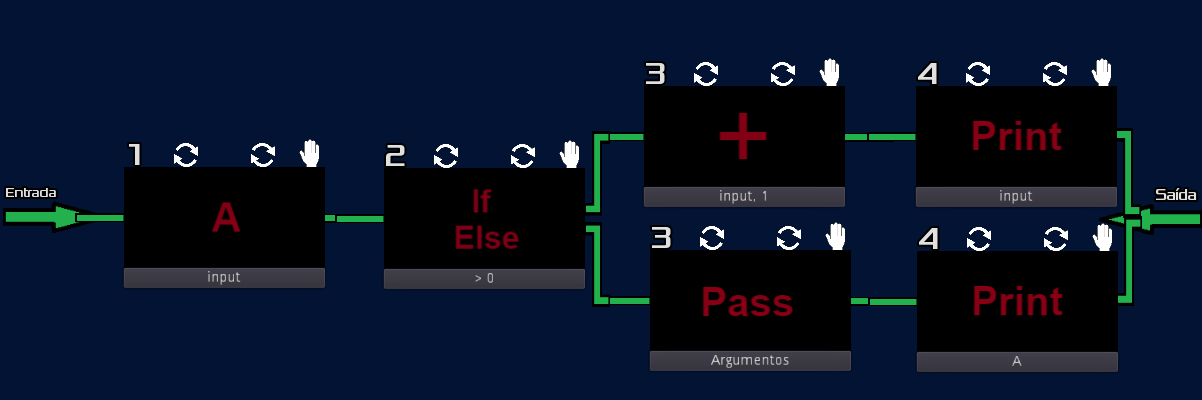
\includegraphics[width=\textwidth]{../figuras/sistema_conectado_arvore_execucao.png}
    \caption{Sistema gerador da Árvore de Execução}
\end{figure}

\begin{figure}[H]
    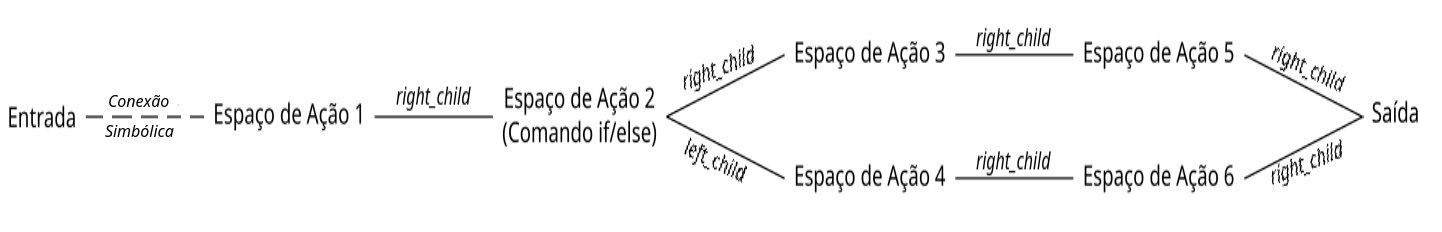
\includegraphics[width=\textwidth]{../figuras/arvore_execucao_redim.png}
    \caption{Esquema de Árvore de Execução}
\end{figure}

Vale ressaltar três pontos importantes:

\begin{itemize}
    \item[$\bullet$]
        A conexão entre a \textit{Entrada} e o primeiro espaço de ação é apenas 
        simbólica, pois a \textit{Entrada} não possui variáveis 
        \textit{right\_child} e \textit{left\_child}. Foi escolhida esta 
        representação de imagem para facilitar o entendimento do leitor que a 
        árvore de execução representa o sistema do jogo, embora dentro do código
        não exista a conexão entre a \textit{Entrada} e o primeiro espaço de 
        ação.
    \item[$\bullet$]
        Os filhos da esquerda, conhecidos como \textit{left\_child}, que 
        não foram representados no esquema, para melhorar a apresentação e 
        deixá-lo mais fácil de entender, existem e possuem o valor 
        \textit{null}.
    \item[$\bullet$]
        A numeração do sistema refere-se a ordem que os comandos serão 
        executados, já a numeração do esquema enumera apenas a quantidade
        de espaços de ação que foram utilizados, portanto as numerações
        podem diferir.
\end{itemize} 

Agora será dada a exlicação sobre a cena \textit{ActionSpace}, parte fixa do 
espaço de ação mostrada na figura 3.9, que é composta pelos seguintes nós:

\begin{itemize}
    \item[$\bullet$]
        \textbf{\textit{ActionShape}} - Delimita, com um retângulo preto, o
        espaço ocupado pelo espaço de ação.  
    \item[$\bullet$]
        \textbf{\textit{Name}} - Coloca o nome "Espaço de Ação" dentro do 
        retângulo preto, pois tutorial faz referências a este item. 
    \item[$\bullet$]
        \textbf{\textit{ArgumentButton}} - Botão que permite ao jogador 
        abrir a área de preenchimento dos argumentos que serão passados para um 
        comando.
    \item[$\bullet$]
        \textbf{\textit{Argument}} - Área de preenchimento dos argumentos, 
        o que for escrito nesta área será passado como argumento para o comando
        posicionado.  
    \item[$\bullet$]
        \textbf{\textit{ArgumentOk}} - Quando pressionado fecha a área de 
        preenchimento dos argumentos.
\end{itemize}

Novamente, vale lembrar que os detalhes de implementação não são relevantes, 
basta saber que esta cena é considerada um recipiente (\textit{container}) para 
o inventário e caso um comando esteja posicionado nesta região não será possível
movimentar o \textit{MovableActionSpace} pela tela.

Uma consideração a ser feita a respeito dos argumentos serem preenchidos 
utilizando o teclado é que um menu de seleção com o mouse limitaria as opções
do jogador, sendo assim ele poderia testar todas as opções disponíveis até que 
uma delas funcionasse, indo contra o objetivo do jogo que é ensinar e não apenas 
terminá-lo. Forçar o usuário a escrever o argumento com o formato pedido faz com
que ele se acostume a ler o menu de ajuda ou as mensagens de erro e seguir os 
padrões que a computação exige, forçando-o a estar ciente do que está fazendo e
concluindo o objetivo principal que é facilitar o aprendizado.

\section{Processo Visual}

Dentro dos arquivos do jogo (diretório \textit{Phoenix Rising}) é encontrado na
pasta \textit{VisualProcess}. Este processo visual trata da animação que auxilia
o jogador a entender o que está acontecendo com os valores do programa durante
a execução.

\begin{figure}[H]
    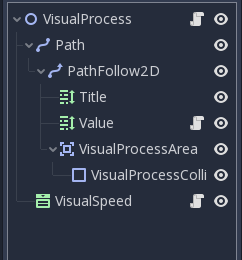
\includegraphics[scale=0.8]{../figuras/cena_visual_process.png}
    \caption{Cena Visual Process}
\end{figure}

\begin{itemize}
    \item[$\bullet$]
        \textbf{\textit{Path}} - Nó que contém a curva de pontos a ser seguida 
        pela parte visual que aparece na tela.
    \item[$\bullet$]
        \textbf{\textit{PathFollow2D}} - Trata dos pontos da curva a ser 
        seguida.
    \item[$\bullet$]
        \textbf{\textit{Title}} - Texto de identificação de qual variável a 
        parte visual está mostrando na tela. (neste projeto apenas é mostrado 
        o valor do \textit{Input})
    \item[$\bullet$]
        \textbf{\textit{Value}} - Valor corrente da variável mostrada pelo
        processo visual que é identificada pelo \textit{Title}.
    \item[$\bullet$]
        \textbf{\textit{VisualProcessArea}} - Área definida para se efetuar a
        mudança dos valores em \textit{Value}, administra alguns parâmetros da
        colisão.
    \item[$\bullet$]
        \textbf{\textit{VisualProcessCollision}} - Área de colisão (utilizada
        pela \textit{Godot}) definida para identificar o momento de se efetuar 
        a mudança dos valores em \textit{Value}.
    \item[$\bullet$]
        \textbf{\textit{VisualSpeed}} - Menu que controla a velocidade que a 
        animação do processo visual será mostrada. 
\end{itemize}

Para entender melhor o processo visual deve-se compreender o básico sobre o
funcionamento dos nós \textit{Path}
\footnote{https://docs.godotengine.org/en/3.1/classes/class\_path.html} e 
\textit{PathFollow2D}\footnote{https://docs.godotengine.org/en/3.1/classes/
class\_pathfollow.html\#class-pathfollow} na \textit{Godot}.
O nó \textit{Path} espera receber uma curva de pontos, já \textit{PathFollow2D}
pega seu \textit{Path}  pai e devolve as coordenadas de um ponto dentro dele, 
dada a distância do primeiro vértice, sendo útil para fazer outros nós seguirem 
um caminho, sem codificar o padrão de movimento. Para isso, os nós devem ser 
descendentes desse nó. Em seguida, ao  definir um deslocamento neste nó, os nós 
descendentes se moverão de acordo.

Seguindo o funcionamento de \textit{Path} e \textit{PathFollow2D} ao instanciar
\textit{Title}, \textit{Value} e \textit{VisualProcessArea} como filhos de
\textit{PathFollow2D} todos eles irão seguir o caminho da curva definida, o que
permite movimentar o valor do \textit{Input} pela tela de jogo. Veja abaixo
algumas variáveis que são utilizadas no controle deste processo:

\begin{figure}[H]
    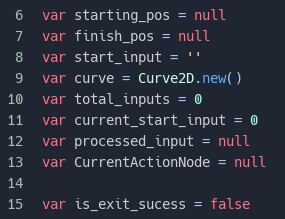
\includegraphics[scale=0.8]{../figuras/variaveis_visual_process.png}
    \caption{Variáveis Visual Process}
\end{figure}

\begin{itemize}
    \item[$\bullet$]
        \textbf{\textit{starting\_pos} e \textit{finish\_pos}} - demarcam onde o 
        processo visual inicia e onde ele termina, respectivamente.
    \item[$\bullet$]
        \textbf{\textit{start\_input}} - recebe o valor inicial da entrada.
    \item[$\bullet$]
        \textbf{\textit{curve}} - guarda a curva 
        de pontos, que será preenchida conforme a execução do programa.
    \item[$\bullet$] 
        \textbf{\textit{total\_inputs}} - guarda a quantidade de valores que foi 
        fornecido na entrada do programa
    \item[$\bullet$]
        \textbf{\textit{current\_start\_input}} - guarda qual valor da entrada que será
        processado.
    \item[$\bullet$]
        \textbf{\textit{processed\_input}} - armazena os 
        valores que se alteram durante a execução e que são exibidos na 
        animação.
    \item[$\bullet$] 
        \textbf{\textit{CurrentActionNode}} - guarda qual espaço de ação que será
        executado
    \item[$\bullet$] 
        \textbf{\textit{is\_exit\_sucess}} - sinaliza se houve algum erro 
        durante a execução.
\end{itemize}

A função que possibilita o processo visual executar as modificações no 
\textit{input} e seguir um caminho na tela é a
\textit{\_on\_MovableActionSpace\_change\_area\_entered} definida no script do
nó \textit{VisualProcess}. Esta função é chamada sempre que há colisão entre 
\textit{VisualProcessCollision} e \textit{ChangeArea}, que está definido no 
espaço de ação.

Veja abaixo o código:

\begin{figure}[H]
    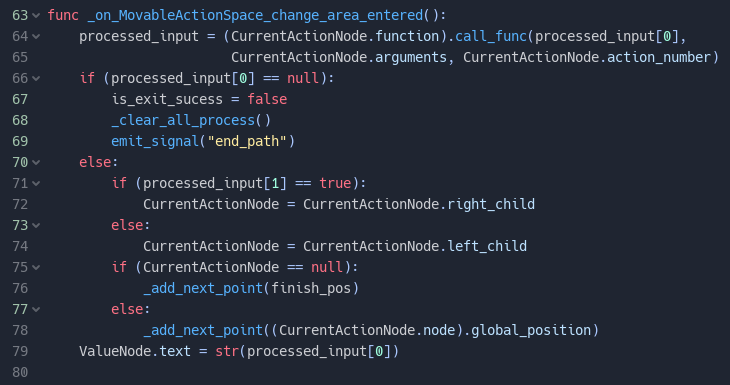
\includegraphics[width=\textwidth]{../figuras/codigo_MovableActionSpace_area_entered.png}
    \caption{Função \_on\_MoveableActionSpace\_change\_area\_entered}
\end{figure}

Note que a função \textit{\_on\_MovableActionSpace\_change\_area\_entered} é 
chamada sempre que é detectada uma colisão entre um espaço de ação e o 
\textit{input}, portanto a variável \textit{CurrentActionNode} está armazenando
uma referência para o espaço de ação que colidiu.

Iniciando a função, na linha 64,
é executado o código do comando que está posicionado dentro do espaço de ação
e o novo \textit{input} que foi processado bem como qual o caminho a seguir,
serão armazenados na lista \textit{processed\_input}.

A lista \textit{processed\_input} guarda, na primeira posição (0), o valor 
resultante da operação do comando posicionado e terá \textit{null} caso algo
tenha dado errado, por exemplo um erro na passagem do argumento. O \textit{if},
na linha 66, verifica se algo deu errado na execução do comando. Caso nada
de errado tenha acontecido é executado o \textit{else}, na linha 70, que
identificará qual será o caminho que o processo visual deverá tomar.

A lista \textit{processed\_input} guarda, na segunda posição (1), qual o
caminho que deverá ser seguido, caso a posição esteja marcada com \textit{true},
então será seguido o caminho do filho da direita, se o valor for \textit{false},
então será seguido o caminho do filho da esquerda. Para entender esta parte
talvez seja necessário relembrar o que significam estes "caminhos" observando 
novamente a figura 3.11: Esquema de Árvore de Execução, definida na seção 
"Espaço de Ação".

Depois há a verificação se o processo visual chegou ao fim, na linha 75, ou 
se há mais algum ponto a seguir, na linha 77-78. Por fim, na linha 79,
atualiza-se o texto que aparece na tela para o jogador visualizar.

Note que a execução dos comandos acontece enquanto o processo visual é mostrado
na tela, assim o jogador pode acompanhar o andamento do seu programa até que
algo de arrado aconteça, facilitando o entendimento de cada comando 
individualmente e a correçao dos erros que aparecerem.

\section{Ambiente de Execução}

Dentro dos arquivos do jogo (diretório \textit{Phoenix Rising}) é encontrado na
pasta \textit{RunEnvironment}. Este ambiente trata de construir o arcabouço 
para executar o sistema.

As imagens abaixo ilustram os nós que compõem a cena principal, chamada 
\textit{RunEnvironment.tscn} e as funções que estão definidas no script
\textit{RunEnvironment.gd} atrelado ao nó principal.

\begin{minipage}[c]{0.5\textwidth}
    \begin{figure}[H]
        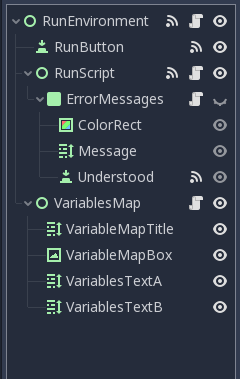
\includegraphics[scale=0.8]{../figuras/cena_RunEnvironment.png}
        \caption{Árvore da cena RunEnvironment}
    \end{figure}
\end{minipage}%
\begin{minipage}[c]{0.5\textwidth}
    \begin{figure}[H]
        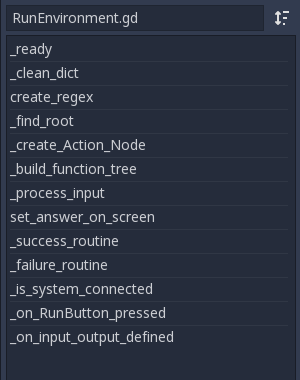
\includegraphics[scale=0.8]{../figuras/funcoes_RunEnvironment.png}
        \caption{Funções de RunEnvironment.gd}
    \end{figure}
\end{minipage}

\begin{itemize}
    \item[$\bullet$]
        \textbf{\textit{RunButton}} - Botão que, ao ser pressionado, faz com que
        inicie uma tenteativa de executar o sistema.
    \item[$\bullet$]
        \textbf{\textit{RunScript}} - Carrega o script \textit{RunScript.gd},
        neste \textit{script} estão as funções de comportamento dos comandos.
    \item[$\bullet$]
        \textbf{\textit{ErrorMessages}} - Espaço definido para a mensagem de 
        erro.
    \item[$\bullet$] 
        \textbf{\textit{ColorRect}} - Dá cor ao espaço destinado as mensagens de 
        erro.
    \item[$\bullet$]
        \textbf{\textit{Message}} - Texto da mensagem de erro.
    \item[$\bullet$]
        \textbf{\textit{Understood}} - Botão que permite fechar a mensagem de 
        erro e dar sequência ao jogo.
    \item[$\bullet$] 
        \textbf{\textit{VariablesMap}} - Carrega o script 
        \textit{VariablesMap.gd}, neste \textit{script} estão as funções que
        dão comportamento ao mapa de variáveis.
    \item[$\bullet$] 
        \textbf{\textit{VariablesMapTitle}} - Título do mapa de variáveis.
    \item[$\bullet$]
        \textbf{\textit{VariablesMapBox}} - Textura destinada ao mapa de
        variáveis.
    \item[$\bullet$] 
        \textbf{\textit{VariablesMapTextA}} - Texto da valoração da variável A.
    \item[$\bullet$] 
        \textbf{\textit{VariablesMapTextB}} - Texto da valoração da variável B.
\end{itemize}

Depois de definir algumas variáveis como o texto do mapa de variáveis e qual a
saída esperada esta cena estará pronta para exercer seu papel mais importante:
\textbf{Iniciar a tentativa de execução do sistema}.

Inicialmente será apenas uma tentativa, pois o sistema pode não estar 
devidamente conectado, impedindo o início da execução ou algum comando pode 
resultar em erro, interrompendo a execução. A ocorrência de ambas as opções 
será explicada a seguir.

Note a função que é chamada assim que o botão \textbf{Rodar!}, definido pelo nó 
\textit{RunButton}, é pressionado.

\begin{figure}[H]
    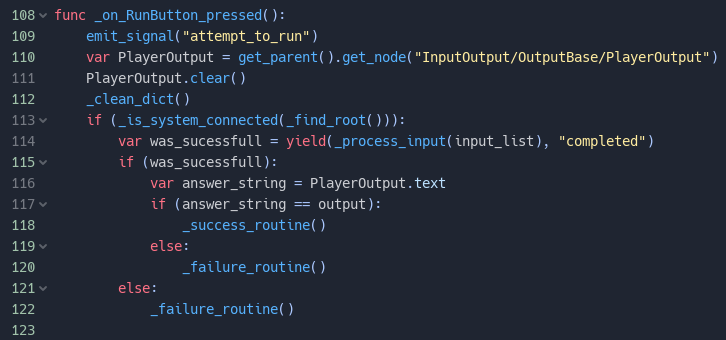
\includegraphics[width=\textwidth]{../figuras/funcao_RunButton_pressed.png}
    \caption{Função do botão \textbf{Rodar!}}
\end{figure}

O sinal emitido na linha 109 serve para armazenar a pontuação no momento em que
o botão é pressionado, assim o jogador ganha os pontos independentemente de 
quanto tempo a animação durou. As linhas 110 a 112 limpam o que estava escrito 
anteriormente na saída do jogador e no mapa de variáveis, para iniciar a nova 
execução.

A verificação se o sistema está conectado é feita pela função 
\textit{\_is\_system\_connected} que recebe a raíz da árvore de execução e
verifica se para todos os espaços de ação que fazem parte do sistema existe 
um caminho que o liga com a saída, sendo que não é válido passar mais de uma vez 
pela mesma conexão.

Veja as figuras abaixo que ilustram um sistema não conectado. 

\begin{figure}[H]
    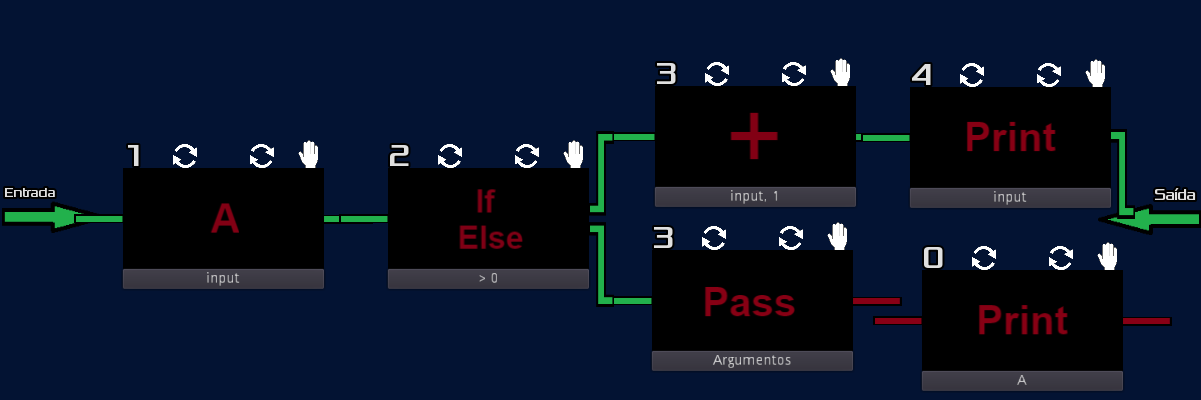
\includegraphics[width=\textwidth]{../figuras/sistema_nao_conectado_arvore_execucao.png}
    \caption{Sistema gerador da Árvore de Execução não Conectada}
\end{figure}

\begin{figure}[H]
    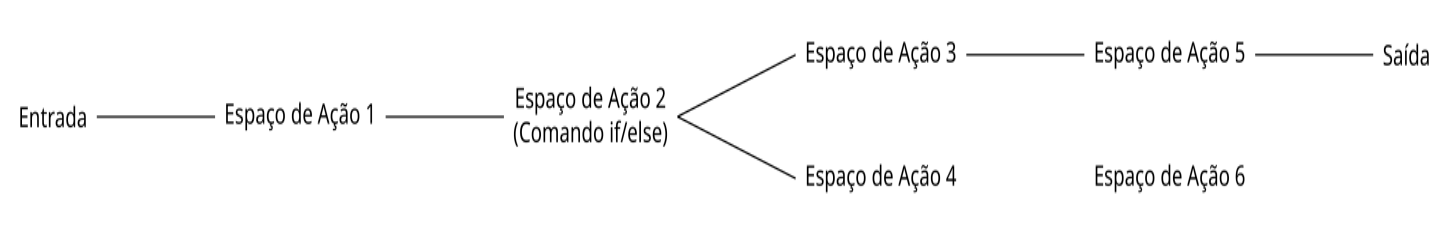
\includegraphics[width=\textwidth]{../figuras/arvore_execucao_nao_conectada.png}
    \caption{Esquema de Árvore de Execução não Conectada}
\end{figure}

Note que o espaço de ação 4 faz parte do sistema, pois existe a conexão 
(caminho) entre a entrada e ele, porém não está conectado com a saída, pois 
não existe um caminho que o ligue com a saída sem repetir uma conexão. Note
também que o espaço de ação 6 não faz parte do sistema, uma vez que não existe
conexão entre ele e a entrada, portanto não é necessário que ele esteja 
conectado com a saída.

Caso seja possível executar o sistema a função que faz o processamento do 
\textit{input} será chamada. Veja abaixo:

\begin{figure}[H]
    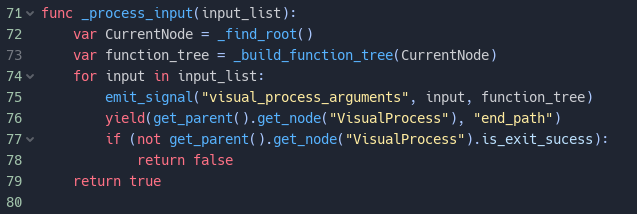
\includegraphics[width=\textwidth]{../figuras/process_input.png}
    \caption{Função \_process\_input}
\end{figure}

Primeiro deve-se encontrar em qual espaço de ação a árvore de execução se 
inicia (linha 72), depois monta-se a árvore de execução completa (linha 73),
por fim a função irá repetir os comandos das linhas 75 a 78 para cada valor
definido no \textit{input}. Para processá-los a linha 75 emite o sinal 
\textit{visual\_process\_arguments} para o processo visual, no \textit{script} 
do processo visual a função chamada por este sinal recém enviado,
\textit{\_on\_RunEnvironment\_visual\_process\_arguments}, preenche os pontos na
curva referentes aos espaços de ação que estão na árvore de execução e inicia a
animação que aparece na tela.

Depois de iniciada a animação o processo visual irá tratar de executar os 
scripts referentes aos comandos que foram posicionados. Enquanto isso a função 
\textit{\_process\_input} estará esperando que o processo visual envie o sinal 
\textit{end\_path}, marcando o fim do processo visual, para prosseguir sua 
execução.

Depois de receber o sinal, a função \textit{\_process\_input} irá verificar se 
o sistema foi executado sem erros ou não e devolver \textit{true} caso o 
sistema tenha sido executado com sucesso ou \textit{false} caso contrário.

Este valor devolvido por \textit{\_process\_input} será armazenado na variável 
\textit{was\_sucessfull}, localizada na linha 114 da função 
\textit{\_on\_RunButton\_pressed}, servindo como verificação se o sistema foi 
executado com sucesso ou não. Caso o sistema tenha sido executado com sucesso a
rotina \textit{\_sucess\_routine} será chamada, adicionando os pontos para o
jogador, fazendo o retângulo de saída piscar em verde e mostrando o botão que 
permite ao jogador ir para o próximo nível. Caso o sistema não tenha sido 
executado com sucesso a rotina \textit{\_failure\_routine} será executada,
piscando o retângulo de saída em vermelho.

Portanto, sempre que o botão \textbf{\textit{Rodar!}} é pressionado estas 
subrotinas serão chamadas e tentarão executar o sistema.

\section{Comandos do Jogo}

Dentro dos arquivos do jogo (diretório \textit{Phoenix Rising}) a declaração 
de quais comandos serão disponíveis é encontrada na pasta 
\textit{GenericGameScenes} no script \textit{ItemDB.gd}, já os comportamentos 
de cada comando estão no script \textit{RunScript.gd} localizado dentro da
pasta \textit{RunEnvironment}.

Para entender como foi estruturado o gerenciamento dos comandos do jogo é 
importante saber que o script \textit{ItemDB.gd} é um \textit{singleton} e é 
carregado antes mesmo que a cena atual se inicie, portanto todas as cenas do 
jogo podem acessar o conteúdo definido nele. Além disso a declaração de cada
comando, feita em \textit{ItemDB.gd}, deve conter 
informações importantes a respeito dele, estas informações são:

\begin{itemize}
    \item[$\bullet$]
        Caminho do ícone referente ao comando, para que as cenas o renderizem
        na tela.
    \item[$\bullet$]
        Texto de ajuda para ser exibido na tela caso o jogador solicite.
    \item[$\bullet$]
        Nome da função que implementa o comportamento do comando.
\end{itemize}

Abaixo está ilustrado uma parte das declarações dos comandos, note que
cada comando possui todas as informações importantes citadas acima.

\begin{figure}[H]
    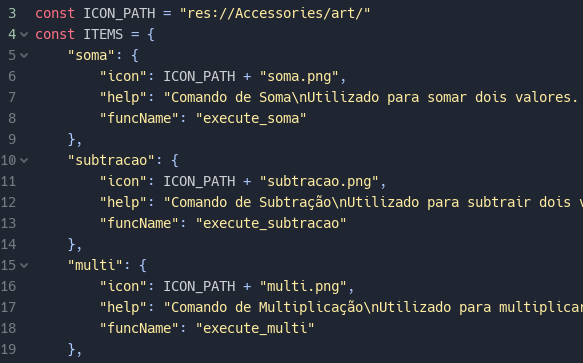
\includegraphics[width=\textwidth]{../figuras/declaracao_comandos.png}
    \caption{Parte do Script de Declaração dos Comandos}
\end{figure}

Para o melhor entendimento desta parte é importante saber um pouco sobre o que é
um dicionário. Basicamente um dicionário é uma forma de estruturar
os dados em que um elemento é chamado de chave e o outro elemento é chamado
de valor. Nele as chaves são únicas e os valores podem se repetir, estes dois
elementos formam um par e ficam atrelados, sendo assim é fácil obter
o valor associado a uma chave apenas utilizando o elemento chave. O necessário
para esta seção é entender que, em um dicionário, podemos utilizar o elemento 
chave para obter facilmente o elemento valor associado.

Na imagem acima a variável \textit{ITEMS} declarada na linha 4 é um dicionário 
e irá armazenar todos os nomes
dos comandos, portanto a chave no dicionário \textit{ITEMS} será a 
\textit{string} que identifica o comando e o valor desta chave será outro 
dicionário que armazena as informações referentes ao comando em questão. Desta 
forma é possível acessar facilmente todas as informações importantes de um 
comando apenas sabendo a \textit{string} de seu nome.

Para recuperar as informações importantes de um comando específico é utilizado 
o mesmo conceito de chave e valor, porém as chaves serão: \textit{icon}, 
\textit{help} e \textit{funcName}.

A única função que está declarada neste script chama \textit{get\_item},
ela recebe o identificador do comando, que no caso será o nome dele, e devolverá
o dicionário que contém as informações importantes dele. Foi criado
um comando chamado "error" que será devolvido pela função \textit{get\_item}
caso o elemento procurado não exista, evitando assim que o programa quebre em 
situações que algo deu errado.

\begin{figure}[H]
    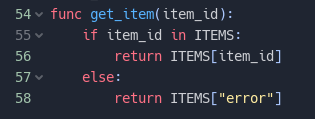
\includegraphics[scale=0.8]{../figuras/funcao_get_item.png}
    \caption{Função get\_item}
\end{figure}

Agora que os conceitos sobre como os comandos são declarados foram explicados é
possível entender como o resto do programa utiliza o que foi definido.

Todos os níveis possuem um \textit{script} atrelado ao nó principal da cena, 
neste \textit{script} exite uma variável chamada \textit{pickup\_item\_list} que
serve para armazenar quais os comandos que serão disponíveis em tal nível. No 
exemplo abaixo estarão disponíveis os comandos de subtração e de \textit{print}.

\begin{figure}[H]
    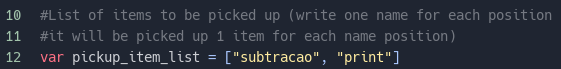
\includegraphics[scale=0.8]{../figuras/item_list.png}
    \caption{Exemplo de pickup\_item\_list}
\end{figure}

Esta lista de itens é passada para o \textit{script} do nó \textit{Inventory}
que utilizará a função \textit{pickup\_item} para colocar cada comando na área 
de comandos e fazê-lo aparecer na tela, note que foi utilizado a chave 
\textit{icon}.

\begin{figure}[H]
    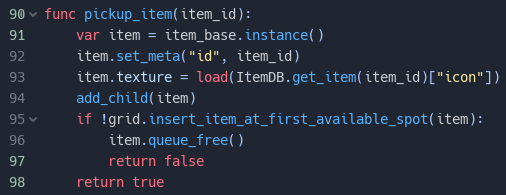
\includegraphics[scale=0.8]{../figuras/pickup_item.png}
    \caption{Função pickup\_item}
\end{figure}

Depois disso o comando estará disponível para ser utilizado, sua
mensagem de ajuda, chamada \textit{help}, será exibida sempre que o jogador 
clicar, com o botão direito do mouse, sobre ele ou quando houver algum 
erro durante a execução do programa devido a sua má utilização.

A última informação importante de um comando é chamada \textit{funcName} e 
guarda o nome da função que implementa o comportamento dele. Os comportamentos
dos comandos estão definidos em \textit{RunScript.gd} e são utilizados durante
a execução do programa que foi criado.

Quando o jogador tenta executar o programa que foi criado a função 
\textit{\_process\_input} chama \textit{\_build\_function\_tree} que 
cria uma árvore com referências para os métodos que definem o comportamento de 
cada item, nesta parte é utilizado o valor em \textit{funcName}. Construída a 
árvore, ela será utilizada pelo \textit{visual\_process} enquanto a animação 
for mostrada na tela. Desta forma é possível executar a função correspondente ao 
comando durante o processo de execução.

Um usuário que queira criar um novo comando só precisará preencher corretamente 
o arquivo \textit{ItemDB.gd} seguindo o modelo e
implementar o comportamento do comando em \textit{RunScript.gd}.

\section{Ajuda ao Usuário}

Dentro dos arquivos do jogo (diretório \textit{Phoenix Rising}) é encontrado na
pastas \textit{UsersGuide} e em \textit{GenericGameScenes}.

Estas cenas formam o conjunto de ajuda ao usuário. Nelas está definido a caixa 
de diálogo, utilizada para guiar o usuário nos primeiros níveis e o painel de 
ajuda que aparece na tela quando o jogador solicita mais informações sobre um 
determinado comando.

A caixa de diálogo exibe mensagens no início do nível dando uma sequência de 
instruções para que o jogador consiga completar o nível mais facilmente. É claro 
que nem sempre essas mensagens irão guiar totalmente o jogador, deixando o 
desafio totalmente nas mãos dele.

Abaixo está um exemplo de mensagem da caixa de diálogo. Esta é uma mensagem que
aparece bem no início do jogo e está ensinando o jogador como fazer para que 
seja possível rodar o programa criado.

\begin{figure}[H]
    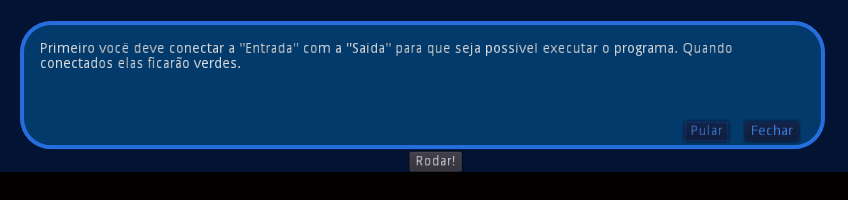
\includegraphics[width=\textwidth]{../figuras/exemplo_users_guide.png}
    \caption{Exemplo de mensagem da caixa de diálogo}
\end{figure}

O painel de ajuda aparece ao clicar, com o botão direito, sobre o 
comando que deseja obter as informações de ajuda. Nele o jogador pode conferir 
o que o comando faz, quais argumentos que ele deve receber e seu modo de 
utilização.

\begin{figure}[H]
    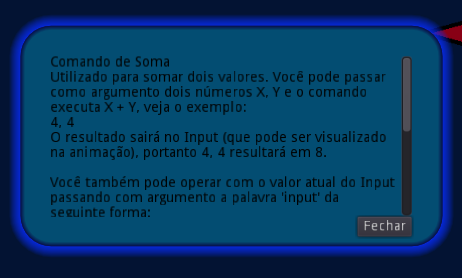
\includegraphics[width=0.8\textwidth]{../figuras/exemplo_help_panel.png}
    \caption{Exemplo de painel de ajuda}
\end{figure}

Como as mensagens da caixa de diálogo devem ser personalizadas para cada desafio, 
existe uma cena no diretório \textit{UsersGuide} chamada \textit{UsersGuide.tscn}
que pode ser instanciada em cada nível. Neste mesmo diretório existe um 
\textit{script} chamado \textit{UsersGuide.gd} que é um modelo para criar as 
mensagens de guia. Portanto, para personalizar as mensagens basta instanciar a 
cena \textit{UsersGuide.tscn} no nível desejado e atrelar a ela um novo 
\textit{script}, seguindo o modelo em \textit{UsersGuide.gd}. Por padrão o nome 
do novo \textit{script} é sempre o nome do nível concatenado com a palavra 
"Guide", ou seja, se o nível chama "NivelX" o nome do script será 
\textit{NivelXGuide.gd}.

A personalização do painel de ajuda para cada comando é feita preenchendo o 
campo \textit{help} ao criá-lo no \textit{ItemDB.gd}.

\section{Gamification}

Dentro dos arquivos do jogo (diretório \textit{Phoenix Rising}) é encontrado na
pasta \textit{Gamification}. Essa pasta contém as cenas e \textit{scripts} que 
gerenciam a transformação da plataforma de ensino em um jogo, ou seja, gerenciam
o processo de \textit{gamificação}.

Cada nível possui um nó \textit{Gamification} que irá gerenciar o sistema de 
pontuação do jogador além de controlar se o jogador já terminou aquele nível
alguma vez durante a sessão de jogo. 

Foi implementado apenas a \textit{gamificação} básica, isto é, em 
\textit{Phoenix Rising} existe apenas o sistema de pontuação. Entretanto 
melhorias podem ser feitas como bônus por número total de tentativas, troca 
de pontos por dicas em níveis difíceis, entre outros chamativos que um jogo 
pode proporcionar. Adicionar novas características de jogo seria um início
interessante para quem gostaria de aprender programação alterando código, pois
além da criatividade, é necessário dominar certas estruturas de dados.

\section{Nível Base}

Dentro dos arquivos do jogo (diretório \textit{Phoenix Rising}) é encontrado na
pasta \textit{BaseLevel}. Dentro dessa pasta está um modelo de nível para ajudar 
alguém que queira construir seu próprio desafio.

A imagem abaixo ilustra os nós que compõem o nível base, nela é 
possível entender sobre a organização dos nós na criação de um novo desafio. 

\begin{figure}[H]
    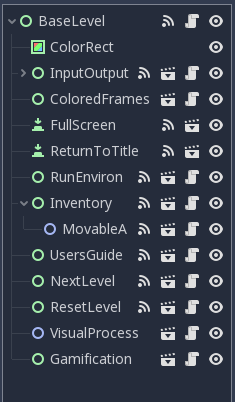
\includegraphics[width=0.6\textwidth]{../figuras/exemplo_base_level.png}
    \caption{Exemplo de nível base}
\end{figure}

Para os interessados em criar um novo nível essa cena é muito útil, pois ao 
abri-la utilizando a \textit{Godot Engine} é possível clicar em cada nó para ver
o destino de cada sinal que é emitido por ele e qual a função que trata o 
recebimento de tal sinal.

Como as cenas mais importantes do jogo já foram explicadas , neste ponto basta
entender como os sinais se conectam no nível base, copiar o diretório
\textit{BaseLevel} e renomeá-lo (incluindo os arquivos dentro dele)
seguindo o padrão "LevelX", depois pode-se editar o desafio a vontade.

Para conectar o novo nível à sequência de jogo deve-se utilizar a função
\textit{\_on\_NextLevel\_next\_level} definida em cada \textit{script}
atrelado ao nó principal do nível. Se quiser adicionar o nível na tela de 
seleção é só checar o diretório \textit{LevelSelection} e seguir os modelos.